\section{Data Placement Algorithm Design}
\label{sec:design}

In this section, we introduce the design of the data placement algorithm. We first present the problem formulation. Then, we present an overview of our algorithm architecture. Finally, we present a detailed description of its components and related algorithms.


\subsection{Problem Formulation}
\label{problemformulation}

The core problem is formulated as follows. Given a set of storage devices represented by HDDs and SSDs as the hardware platform, our task is to find a data placement that 1) satisfies user polices on data placements, and 2) maximizes the throughput of I/O operations from HPC applications. This problem is challenging due to: 1) we don't have complete knowledge on future access patterns to data objects due to the dynamics of workloads, 2) user policies can be highly heterogeneous and may change over time. Therefore, if we model such a problem as an optimization problem, its solution is from a very large search space, such that it is very hard to always reach the optimal configuration when something changes, even such change could be slight. Furthermore, given that the users' request may change frequently, we would like to be able to re-use previous calculation results as much as possible, so that we can avoid the re-calculation when a similar scenario is met in practice.


%ased on such concerns, we formulate the following problem: \textbf{given the underlying demands, how can we find an optimized storage placement that can incrementally provide results that can achieve the best performance under the resource constraints and user requirements?} Note that given that the users' request may change frequently, we would like to be able to re-use previous calculation results as much as possible, so that we can avoid the re-calculation when a similar scenario is met in practice.

\begin{figure}[t]
\begin{centering}
  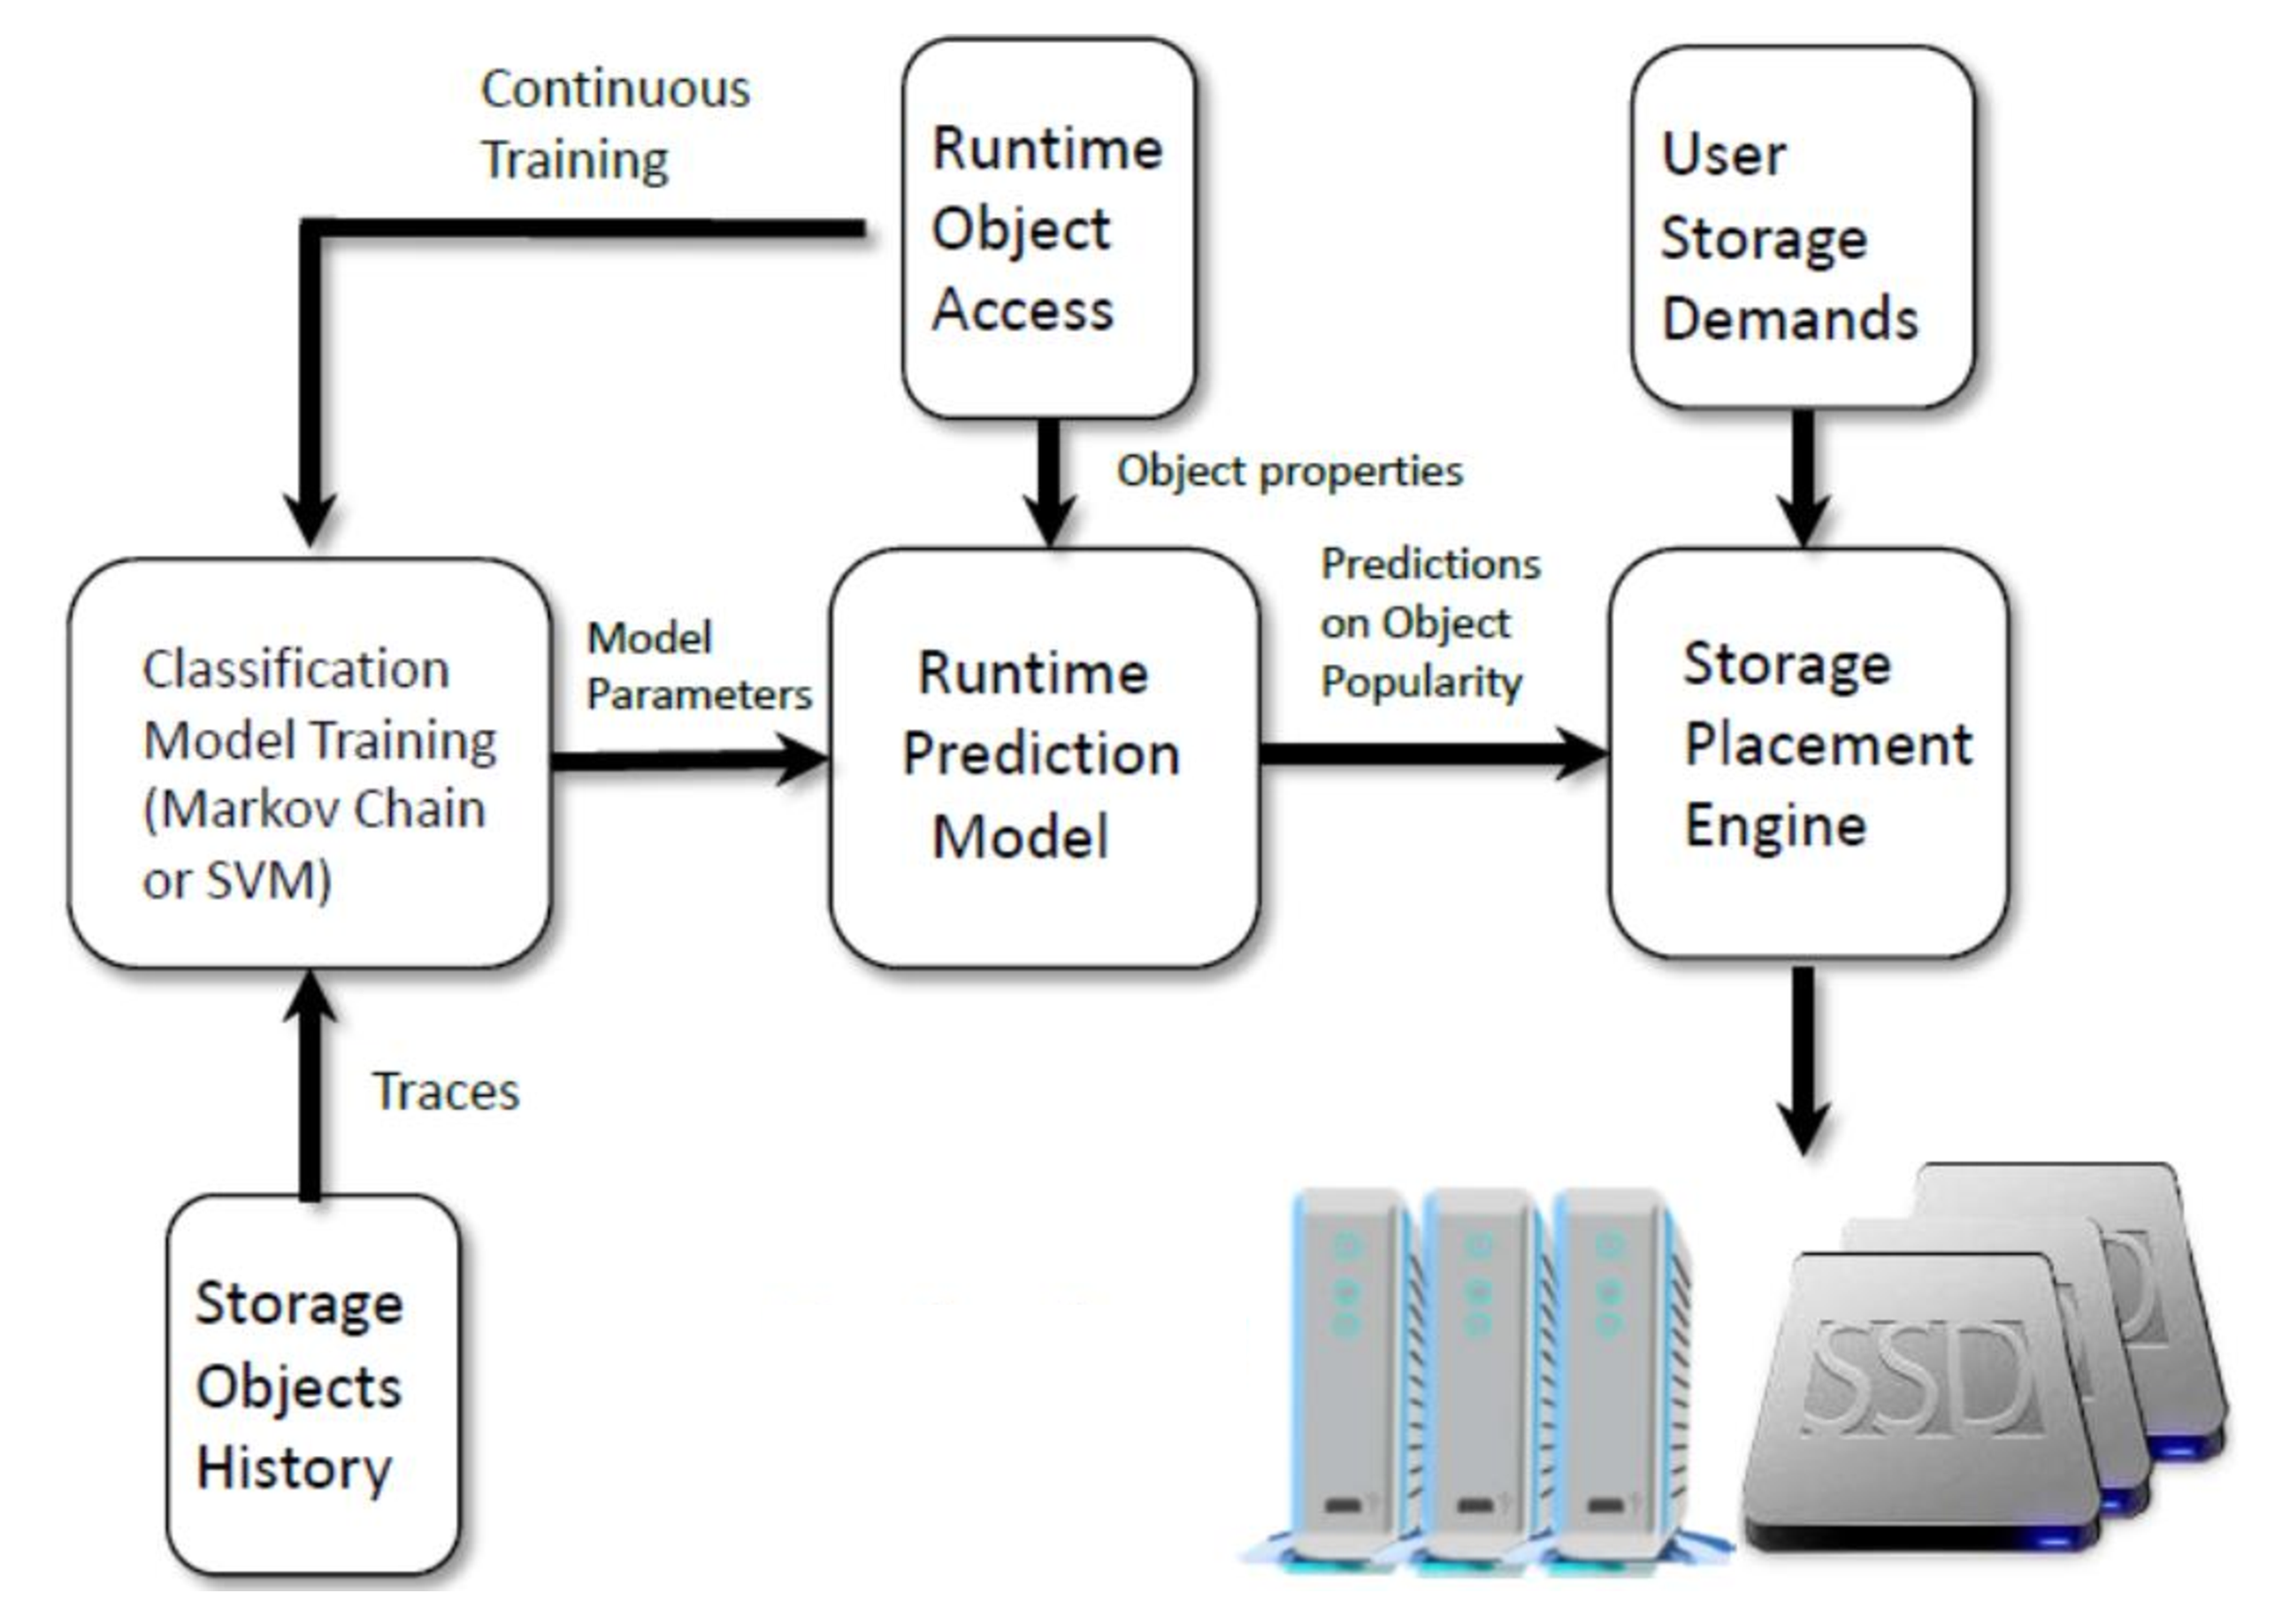
\includegraphics[width=2.3in]{./arch.pdf}
  \caption{The Design Architecture}\label{fig:architecture}
  \label{arch}
\end{centering}
\vspace{-0.1in}
\end{figure}






\subsection{Architecture Overview}
\label{architecture}


We first present the design architecture of our data placement algorithm. For this design, we consider the I/O workload from user applications to include both read and write operations. All I/O workload are generated to access data objects, which are minimal storage units in object-based storage systems. In practice, a large file can be divided into multiple data objects which will be stored on single or multiple object-based storage devices (OSDs). Note that the write operations may be dominating for certain I/O workload, such as periodic checkpoint~\cite{naksinehaboon2008reliability}. The I/O workload from user applications may also change over time, therefore, the solution should adapt to the dynamic nature of the I/O workload.

Figure~\ref{arch} shows the overall architecture, where the whole procedure works as follows: the first core component, the classification model, is trained based on the access history of data objects. In our current work, we concentrate on the historical access frequency of data objects, while we leave exploiting the access pattern (sequential/random read or write) to improve data placement performance as our future work. After training, it provides parameters for the runtime prediction model that are used to predict the access popularity of data objects in the future. Specifically, the predictions decide if an object is going to have ``recurring'' or ``non-recurring'' accesses, based on its history of accesses, as well as the particular workload that accessed them. Such predictions are then used, together with user demands, as the input for the storage placement engine, whose goal is to generate an optimized placement of data objects to storage devices so that the overall system level performance on access delay and bandwidth can be improved. Finally, the runtime object access traces are also used as input for the classification model for continuous training purposes, and keeping the parameters up-to-date.


\subsection{Markov Chain based Workload Classification}

In this section, we describe how the classification model generates model parameters based on object access traces. In our design, we adopt a Markov chain based approach. %Formally, we first select a list of features for a data object for training purposes. Suppose that we select an $N$-tuple that forms a workload signature as:

%\[
%  Signature = {m^1, m^2, ..., m^n}
%\]
%
%where the $m^i$ represents a measured metric of $i$. Note that the metric selection process is fully automated and transparent to the user. The particular $m^i$ may have flexible semantics, and for our present purpose, we focus primarily on its metric of access frequency.

%Once the signatures are collected, it is important that we can classify later workloads based on the training periods. This is based on the assumption that user workloads will have inherent repeating patterns, where similar workloads may be encountered again. This therefore resembles the ``cache hit rates'' which are well studied in the computer cache designs. But still there are considerable differences, as unlike cache contents, the workload signatures may indeed shift over time. Therefore, it is only giving approximate solutions, not accurate answers.

Observe that there exists a tradeoff in the overhead of training and the prediction accuracy. Therefore, we need to achieve a good tradeoff in our design. Our approach has the following key steps. First, we assume that we can keep the access history for each data object. In reality, it may not be practical to record a long access history for each data object since in that case the storage overhead could be huge, instead, only recent access history needs to be maintained and updated periodically. Second, we model the access frequency of each data object using a discrete-time Markov chain in which each state represents a specific range of access frequency. With the access history, we can estimate the parameters of the Markov chain model. Third, by calculating the stationary distribution of the Markov chain, we can predict the likelihood for the access frequency of each data object to stay within certain ranges in the long run. Finally, we rank each data object based on the weighted sum of the stationary distribution, where the weights are chosen according to the specific range represented by each state in the Markov chain. A higher rank of the data object indicates that it is more appropriate and efficient to be moved or placed into low-latency, high-bandwidth drives such as SSDs. We next describe these steps in more detail.

\subsubsection{Collection of Access History of Data Objects}


\begin{figure}[!t]
\centering
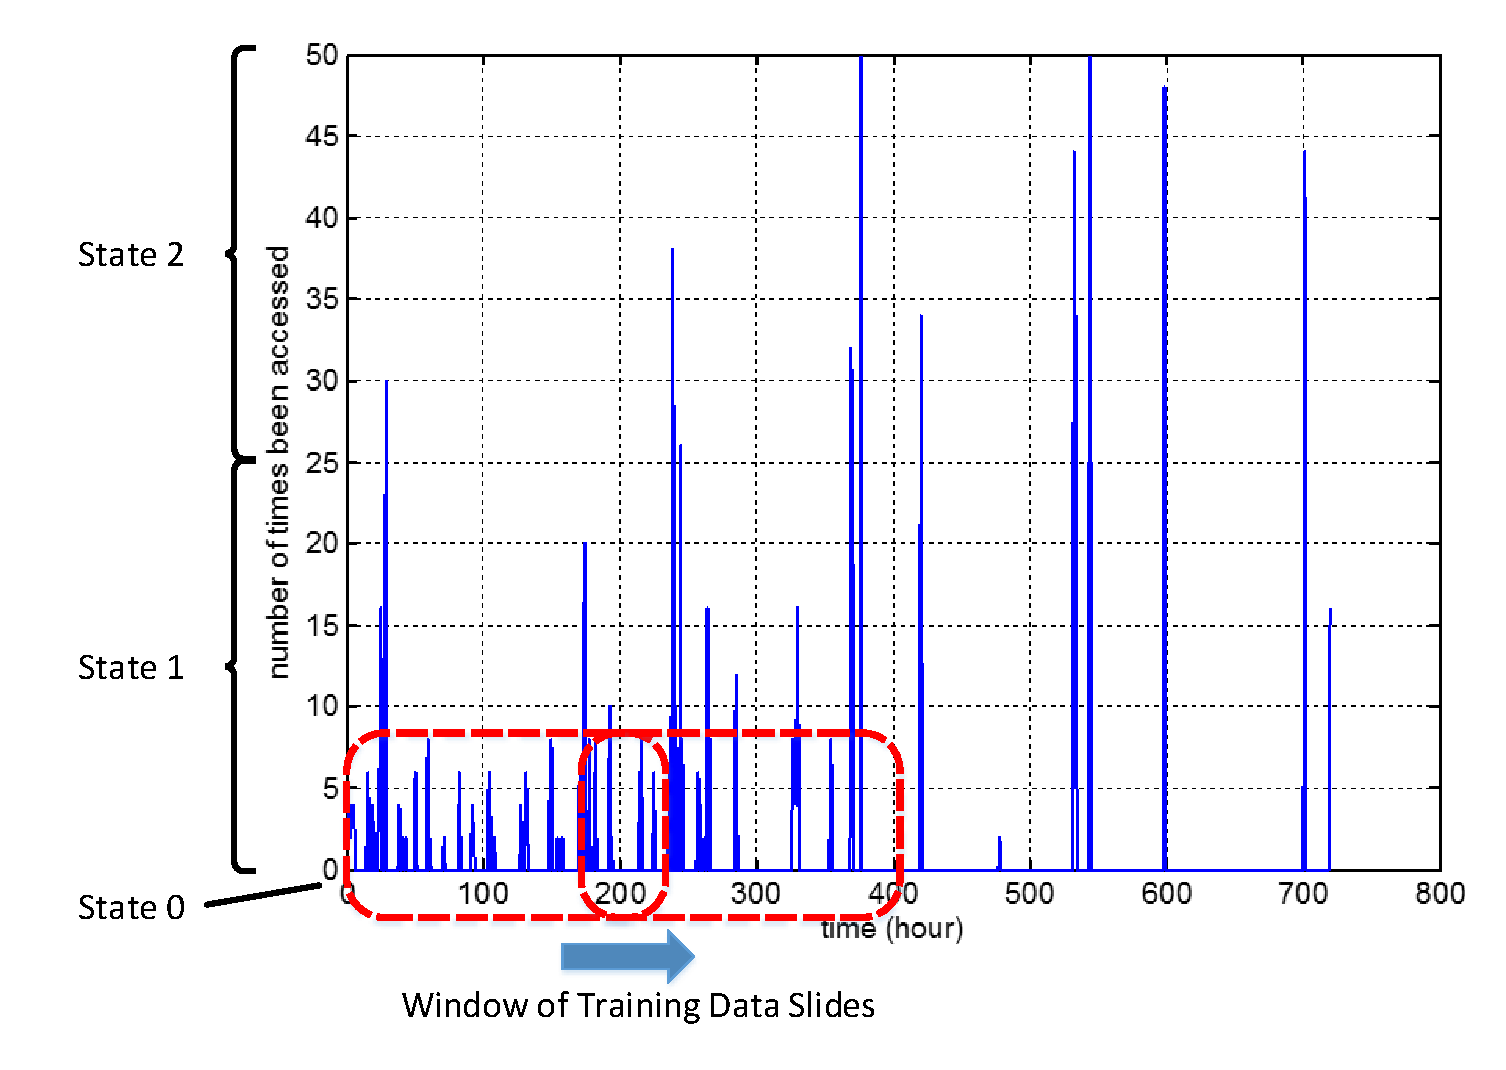
\includegraphics[width=3.0in]{./trace.pdf}
% where an .eps filename suffix will be assumed under latex,
% and a .pdf suffix will be assumed for pdflatex; or what has been declared
% via \DeclareGraphicsExtensions.
\caption{Traces of Data Object Accesses in Frequency}
\vspace{-0.25in}
\label{trace}
\end{figure}


Fig. \ref{trace} demonstrates the access frequency (here the ``access'' includes both read and write operations) of a data object during one month from the LASR traces~\cite{tracedata2}, which include I/O activities of benchmark applications for the SEER project, which observes users' file access patterns across storage networks. The X axis of Fig. \ref{trace} is the range of one month time that has been divided into 720 time periods (each period is 1 hour). The Y axis represents the number of times the data object has been accessed during each time period. As the storage overhead for maintaining the entire access history of each data object is not cost-effective, we only maintain recent access history of each data object and use such access history to build a Markov chain model to predict the future access frequency. As shown in Fig. \ref{trace}, only the access history in the dotted window is used to train the prediction model, where the window will slide with time so that we can implement online prediction for data objects access frequency.

\subsubsection{Markov Chain Predication Model}

With the access history of each data object, we build a Markov chain model to predict the future access frequency of data objects. First, we need to determine how many states the Markov chain should have and the range of access frequency each state represents. For example, as shown in Fig. \ref{trace}, if the maximum number of access times during an observation period is 50, then, for example, we can divide 50 evenly into two ranges, and build a Markov chain model that has three states: $0$, $(0,25]$, and $(25,50]$, respectively. If during a time period, there is no access of the data object, then the Markov chain will stay in state 0. If the number of access times is larger than 0 but less than 25, then the Markov chain will stay in state 1, and so on. The transition diagram of the Markov chain is shown in Fig. \ref{transitioin}.

\begin{figure}[!t]
\centering
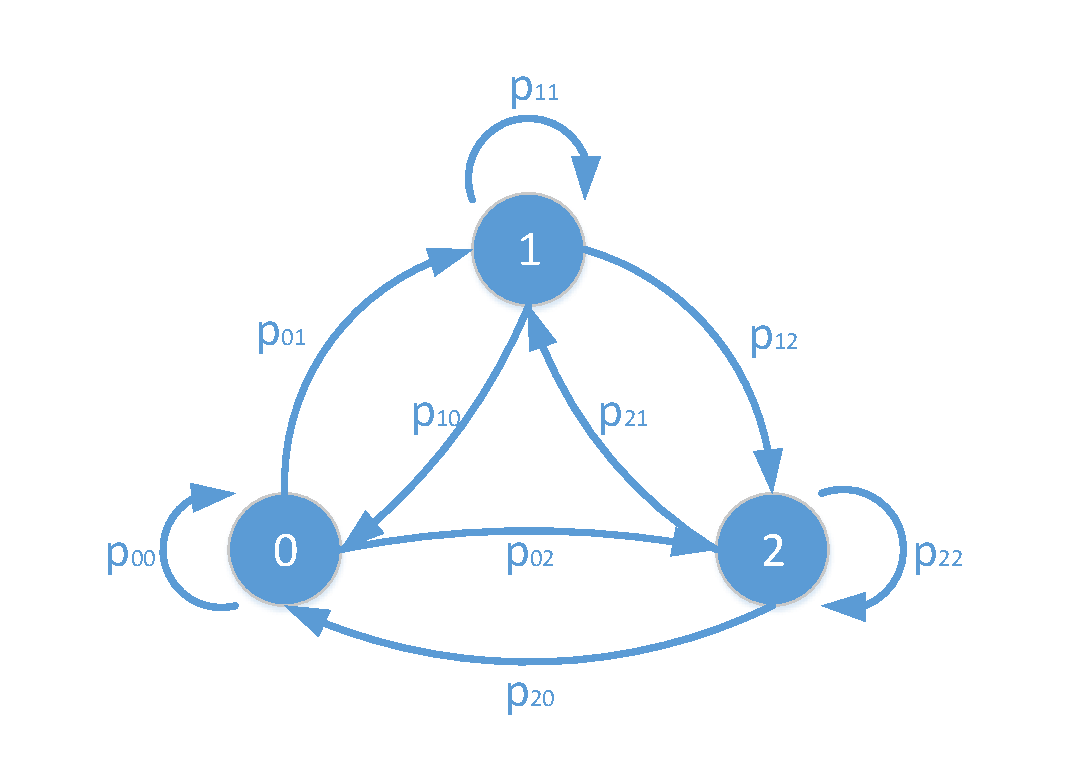
\includegraphics[width=1.9in]{./transition.pdf}
% where an .eps filename suffix will be assumed under latex,
% and a .pdf suffix will be assumed for pdflatex; or what has been declared
% via \DeclareGraphicsExtensions.
\caption{Transition Diagram of Markov Chain}
\vspace{-0.25in}
\label{transitioin}
\end{figure}

Second, we transform the access history to the state transition sequence of the Markov chain based on the specific range each state represents. For example, after transformation the state transition sequence of access history shown in Fig. \ref{trace} is: 1,1,1,1,1,0,0...  Based on this state transition sequence, we can estimate the transition probabilities between every two states and construct the transition matrix of the Markov chain shown below:

\begin{equation}
\mathbf{T} =
 \begin{pmatrix}
  p_{00} & p_{01} & p_{02} \\
  p_{10} & p_{11} & p_{12} \\
  p_{20} & p_{21} & p_{22}
 \end{pmatrix}
\end{equation}

According to the properties of Markov chain, we have:
\begin{equation}
\lim_{n\to\infty}\mathbf{T}^{n} =
 \begin{pmatrix}
  \pi_{0} & \pi_{1} & \pi_{2} \\
  \pi_{0} & \pi_{1} & \pi_{2} \\
  \pi_{0} & \pi_{1} & \pi_{2}
 \end{pmatrix}
\end{equation}
in which $\boldsymbol{\pi} = [\pi_{0}, \pi_{1},  \pi_{2}]$ is called the stationary distribution of the Markov chain. We can simply calculate $\boldsymbol{\pi} $ through computing a normalized multiple of a left eigenvector $\mathbf{E}$ of the transition matrix $\mathbf{T}$ with an eigenvalue of 1:
\begin{equation}
\boldsymbol{\pi} = \frac{\mathbf{E}}{\sum_{i}e_{i}}
\end{equation}
where $e_{i}$ is the $i$-th element of eigenvector $\mathbf{E}$. Since the stationary distribution $\boldsymbol{\pi}$ reflects the probabilities that each state of Markov chain will be visited in the future, which can be used to predict the access frequency of each data object.

Based on the predicted access frequency in the future, we rank the data objects  so that we can determine which data object should be placed or moved to SSD drives. Note that, however, even if the calculated stationary distribution tells us state 1 will be visited with higher probability than state 2, to rank the importance of the data object, we must consider that state 2 represents a higher access frequency. Therefore, we use a weighted sum of the stationary distribution to rank the importance of the data objects, where the weights are defined by values that are proportional to the access frequency ranges that the states represent. For example, if we obtain the stationary distribution of the data object as $\boldsymbol{\pi} = [0.31, 0.56, 0.13]$, and we assign weights $[0, 10, 20]$ to the three different states, we can calculate the rank of the data object by $rank_{obj_{x}} = 0.31\times0+0.56\times10+0.13\times20 = 8.2$. We can then compare the ranks of objects, and provide input for the placement engine.

\begin{table}[t]
\centering
\scriptsize
\begin{tabular}{|l|l|}
\hline
 $N$ & Total number of storage drives \\
 \hline
 $M$ & Total number of data objects  \\
 \hline
 $cs_i$ & Capacity of storage drive $i$ \\
 \hline
 $ds_i$ & Size of data object $i$\\
 \hline
 $f_i$ & Predicted frequency of access for data object $i$\\
 \hline
 $b_{ij}$ & Bandwidth for the link connecting storage drives $i$ and $j$\\
 \hline
 $at_i$ & Average throughput for storage drive $i$\\
 \hline
 $e_{ij}$ & Whether data object $i$ is stored on storage drive $j$ ($0$ or $1$)\\
 \hline
 $cp_i$ & The minimum number of copies for data object $i$\\
 \hline
\end{tabular}
\normalsize
\caption{Notations of Symbols}
\vspace{-0.3in}
\label{tablenotes}
\end{table}


\subsection{Finding Placements under User Polices}

Once we obtain the predicted popularity of data objects, i.e., their ranks, the next step is to find an optimized placement solution such that the access latency is minimized, while satisfying users' placement policies. In this aspect, we assume that users' requests will be parametric, meaning that all requests will be embedded into equations or constraints. For example, by using the notations in Table~\ref{tablenotes}, a requirement on the number of redundant copies of a data object $i$ stating that at least three extra copies must be made can be expressed as $cp_i > 3$.

Our solution to this problem is by formulating the placement problem in a mathematical optimization as follows:

We want to maximize:

\begin{equation}
\sum\limits_{i \in M} f_i \times max[\forall j \in N, at_j\times e_{ij} ]
\label{goalmetric}
\end{equation}

subject to constraints such as:

\begin{equation}
\sum\limits_{j\in N} e_{ij} = cp_i, \forall i \in M,
\label{capacity}
\end{equation}

\begin{equation}
\sum\limits_{\forall i \;\; s.t.\;\; e_{ij} = 1} ds_i \le cs_j, \forall j \in N, \label{duplicate}
\end{equation}

In this short paper, we only give a description of an easier scenario in these equations. In this example, Equation~\ref{goalmetric} specifies that we want to find a way that assigns data objects to storage devices such that the weighted access throughput by the access frequency is maximized.  Note that we use the equation $at_j\times e_{ij}$ to filter those storage devices where the particular data object $i$ is stored on: if $i$ is stored on device $j$, we know $e_{ij}=1$, otherwise $e_{ij}=0$. Hence, finding the $max$ of them translates into finding the storage unit with a copy of data object $i$ that has the highest throughput.

On the other hand, this optimization goal is subject to two or more constraints. In this example, we only consider two of them, in Equation~\ref{capacity} and Equation~\ref{duplicate}, respectively. The first constraint specifies that each storage drive $j$ should not contain more data objects than its capacity, while the second constraint specifies that the number of duplicate copies of a data object should be set according to the users' placement polices. If a data object does not need to have duplicates, its $cp$ value is set to $1$ by default.

In more complex scenarios, the users may have additional constraints. As we mentioned earlier, such constraints are parameterized, meaning that we can easily add more constraints to the formulation above. Finally, even the optimization goal can be adjusted. For example, if we only want to minimize the access delay rather than the throughput, we can change the Equation~\ref{goalmetric} accordingly.

Based on this formulation, we notice that the optimization is reduced to a linear programming problem where we can use numerical methods to recalculate its solution periodically in the placement engine. Note that the engine is operating independently of the rest of the system. Doing so does not require the engine to be tightly integrated, so that we can easily change the engine's implementation as needed, which gives us additional flexibility.

